\chapter{Trabalho relacionado} \label{cap:trabrelacionado}

Compete, neste cap��tulo, explanar o estado da arte em cada uma das
vertentes do trabalho, por forma a sustentar a discuss�o da adequabilidade da
solu��o proposta. Sabendo que a componente de an�lise cr�tica � de indispens�vel
presen�a num trabalho cient�fico, procurar-se-�, sempre que oportuno, acompanhar
as explica��es com uma interpreta��o t�cnica, como forma de justificar as
op��es efectuadas face  pan�plia de alternativas existentes na academia.
\section{Desenho e Implementa��o de RSSF Seguras }
\label{sect:sec_secure_wsn_design}
Sendo o tema central do trabalho proposto o estudo das propriedades de
seguran�a nestas redes, importa, em primeiro lugar, perceber, de forma
consistente, a sua arquitectura de protocolos. Em segundo lugar, � necess�rio
entender quais os servi�os de seguran�a disponibilizados, por forma a
poder adequar-se �s aplica��es para as quais s�o criadas
e desenhadas as RSSF.
\subsection{Arquitectura de uma RSSF}
\label{sect:subsec_arq_sofware_wsn}
As redes de sensores t�m uma arquitectura considerada minimalista porque, ao
contr�rio de outras arquitecturas de redes, est�o organizadas em menos camadas,
fundindo algumas fun��es desempenhada por camadas inferiores para outras
superiores ( ex: a camada de aplica��o pode desempenhar algumas fun��es da
normalmente atribu�das � camada de transporte). Assim, � fundamental perceber
qual a pilha de protocolos que as RSSF implementam, bem como perceber quais os
sistemas que comp�em um sensor gen�rico para de seguida apresentar algumas
implementa��es de sensores.
\subsubsection{Modelo da plataforma gen�rica de uma RSSF - \textit{Mote}}
� semelhan�a do que acontece com as redes convencionais, existem n�s de
computa��o interligados por uma infraestrutura de comunica��o. No caso da RSSF,
esta infraestrutura corresponde a comunica��o \textit{multi-hop} em que cada n�
da rede (\textit{mote}) pode desempenhar pelo menos tr�s papeis: 1) N� gerador
de dados, pela capta��o da eventos associados �s especificidades dos sensores
possu�dos; 2) N� encaminhador, que recebe dados de outros n�s e os passa a
outros n�s por forma a que alcance o destino; 3) N� de sincroniza��o ou n� de
agrega��o, embora estas duas caracteriza��es n�o correspondam � mesma tarefa
por si s�, a um n�vel mais macro, corresponde igualmente a colec��o de dados da
rede oriundos da detec��o de eventos, por forma a faze-la seguir agregada para
outro destino (interno ou externo � rede ).

Desta forma interessa perceber qual o modelo inerente a estas pequenas
plataformas de rede que apesar das caracter�sticas limitadoras da sua execu��o
conseguem executar uma complexidade de aplica��es tendo em conta sempre as
limita��es impostas pela arquitectura. Na figura seguinte apresent-se um
modelo \cite{ MODELO_SENSOR} que ilustra os diversos componentes que concorrem
para a efectividade de servi�o de um \textit{mote} numa RSSF.
\begin{center}
\begin{figure}[ht]
\centering
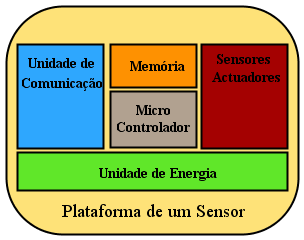
\includegraphics[height=5cm,width=7cm]{SENSOR_NODE.png}
\caption{Modelo de um Sensor de uma RSSF (baseado em
\cite{LIVROARCH_WSN})} \label{fig:sensor_mode}

\end{figure}
\end{center}
Como se pode observar pela figura, da qual se pode generalizar o modelo de uma
plataforma gen�rica de RSSF, os sistemas que est�o presentes s�o os seguintes:
i) Sistema de processamento;ii) Sistema de energia; iii) Sistema de
comunica��o; iv) Sistema sensorial; v) Sistema de mem�ria.
\subsubsection{Arquitectura de \textit{Software} }
Uma das vis�es estruturais da uma RSSF, � a que apresenta pelas camadas de \textit{software} que a
comp�e. Esta vis�o permite ver a plataforma sobre a forma de um conjunto de servi�os que
desempenham tarefas especificas e que lhes permite em cada camada adequar os mecanismos intrinsicos
ao funcionamento, observe-se a figura seguinte que representa esta arquitectura, comparada com o
modelo tradicional das redes 802.2.

\subsubsection{Pilha de Protocolos de uma RSSF }
Uma arquitectura para a a pilha de protocolos em RSSF foi proposta por
\cite{Akyildiz2002}, esta pilha apresenta-se representada por cinco camadas:
\paragraph*{Camada F�sica.}� respons�vel por selec��o de frequ�ncia, detec��o de sinal e modula��o
tendo a minimiza��o do consumo de energia como uma prioridade;
\paragraph*{Camada de Liga��o de Dados.} Das tarefas associadas a estacamada destacam-se as
seguintes: multiplexa��o de dados, acesso ao meio, detec��o de erros/colis�es e detec��o de frames.
Uma RSSF pode ter um protocolo de MAC espec�fico(ex: B-MAC\cite{BMAC}, S-MAC \cite{SMAC}) de modo
agerir o consumo de energia consoante aos protocolos das camadas superiores;
\paragraph*{ Camada de Rede.} sendo a energia um tema transversal a toda a pilha,
esta camada deve endere�ar esta preocupa��o tamb�m, tem como tarefa prim�ria decidir quais os n�s a
escolher para o encaminhamento das mensagens. Um dos sistemas de encaminhamento mais simples � o
baseado na inunda��o (\textit{flooding}), no entanto, apesar da simplicidade n�o tem alguns
problemas como por exemplo: a duplica��o de mensagens e a total ignor�ncia dos recursos da rede,
nomeadamente os energ�ticos. Um dos protocolos que minimiza o impacto da inunda��o � o
SPINS\cite{REF}, negociando e adaptando-se aos recursos existentes;
\paragraph*{Camada de Transporte.} Nas redes convencionais � respons�vel pela  gest�o da congest�o
de tr�fego na rede, gest�o da fiabilidade da comunica��o. Nas RSSF normalmente aparece, muitas
vezes, integrada com  a camada aplica��o
\paragraph*{Camada de Aplica��o.} V�rias s�o as aplica��es desenvolvidas para esta camada,
normalmente, est�o associadas �s capacidades sensoriais das plataformas, que naturalmente est�o
relacionadas com o fim para o qual se instala/desenha a RSSF.

INTRODUZIR AQUI A IMAGEM DA PILHA E DOS SERVI�OS

%Tendo em conta as caracter�sticas das RSSF, toda a pilha � acompanhada transversalmente por
%tr�s planos, que devem ser atendidos por cada uma das camadas, de forma a
%lidarem de forma optima com a energia, mobilidade e recursos partilhados, e
%estes s�o os seguintes: plano de gest�o de tarefas , plano de gest�o
%de energia e plano de gest�o de mobilidade. 
%Esta camada surge com maior relevo quando importa a
%uma infraestrutura de RSSF comunicar com uma rede exterior. No entanto algumas
%das tarefas que podem ser desempenhadas por esta camada acabam por ser
%desempenhadas pela camada de aplica��o, j� que normalmente dizem respeito
%a qualidade de servi�o ou certeza de entrega de  pacotes no destino.
% 
\paragraph{Sistemas de energia}
Como j� tem sido salientado ao longo deste trabalho e pode ser encontrado em
qualquer texto sobre RSSF, a energia � um recurso escasso e como tal deve ser
tomado em conta no desenho de redes de sensores, dependendo tamb�m da aplica��o
ou dos eventos que se pretendem monitorizar bem como a frequ�ncia com que estes
se verificam. Assim, os dispositivos fornecedores de energia podem ser de
diversos tipos, por exemplo: baterias (tipo AA), baterias solares.
Encontra-se nas especifica��es das plataformas mais recentes os valores que
indicam o consumo energ�tico nos diversos estados de opera��o de um
\textit{mote} a titulo de exemplo observe-se a plataforma 
\textit{Mica2}\cite{MICA} da \textit{Crossbows}\cite{CrossbowSite}:
\begin{table*}[ht]
\centering % used for centering table
\begin{tabular}{l r} % centered columns (4 columns)
\hline\hline %inserts double horizontal lines
Descri��o & Valor \\ [0.5ex] % inserts table
%heading
\hline % inserts single horizontal line
Baterias& 2xAA \\ % inserting body of the table
M�nimo $V_{in}$ & 2.7 V \\
Capacidade da bateria& 2000 mAh \\
Regulada &  no \\
\hline %inserts single line
\end{tabular}
\label{table:mica2_caracter} % is used to refer this table in the text
 \caption{Caracter�sticas de energia do \textit{mote} Mica2
(origem:\cite{SNMuseum}))} % title of Table
\end{table*}



\begin{table*}[ht]
\centering % used for centering table
\begin{tabular}{l r} % centered columns (4 columns)
\hline\hline %inserts double horizontal lines
Opera��o & Consumo\\ [0.5ex] % inserts table
%heading
\hline % inserts single horizontal line
CPU \textit{sleep} com \textit{timer} \textit{on} & 0.054 mW \\ % inserting body
CPU activo,\textit{ radio }\textit{off} & 36 mW \\
CPU activo, \textit{radio idle listening }& 66 mW \\
CPU activo, \textit{radio TX/RX }& 117 mW \\
Pot�ncia M�xima (CPU activo, radio TX/RX + flash write) & 165 mW \\ [1ex] %
%[1ex] adds \hline %inserts single line
\end{tabular}
\label{table:mica2_powerops} % is used to refer this table in the text
 \caption{Consumo de Energia \textit{Mica2} - Opera��o Tipica
(origem:\cite{SNMuseum})} % title of Table
\end{table*}
\paragraph{Sistemas de processamento}
O sistema de processamento � um componente essencial num \textit{mote}
\cite{Holger_Karl_protocols_andarchs_wsn}. � respons�vel por recolher
informa��o de todos os sensores do n� process�-la em conformidade, tem ainda de
tratar a informa��o recebida de outros n�s vizinhos. Toda o conjunto de
processamento pode ser realizado nas v�rias arquitecturas representando um
\textit{trade-off} entre desempenho, flexibilidade, performance, custo e
consumo de energia. � semelhan�a do que acontece com os processadores de
computadores convencionais existem microprocessadores gen�ricos que podem ser
aplicados nas mais variadas aplica��es, em especial estes processadores podem
entrar em modos de consumo reduzido (passando para o estado \textit{sleep})
quando n�o est�o a efectuar processamento. Dois dos processadores mais
utilizados nas redes de sensores actuais s�o os da tecnologia Atmel Atmega 128L
\cite{atmel} e da Texas Instruments o controlador TI MSP430 \cite{TIMSP430}

\paragraph{Sistemas de comunica��o}
Este sistema � o respons�vel pela transfer�ncia de dados entre diversos n�s de
uma rede, no caso das RSSF, este sistema � de radio frequ�ncia que permite
dispor de uma rede sem necessidade de infraestrutura de cabos. A
r�dio-frequ�ncia permite ter bom alcance de comunica��o com boas taxas de
transfer�ncia, bem como equilibrar o consumo de energia perante exist�ncia de
erros. Assim para o uso efectivo deste tipo de comunica��o � necess�rio
escolher bem a gama de frequ�ncia de opera��o que tipicamente se situam entre
as gamas 433 Mhz e 2.4Ghz.

Componente ainda fundamental � a existencia de transmissores e receptores
\footnote{No caso da implementa��o em RSSF, as plataformas incorporam num
mesmo componente as duas fun��es, transmiss�o e recep��o, estes s�o denominados
por \textit{transceivers}}nos
n�s. Estes t�m a fun��o de transformar uma cadeia de bits, vindas do
processador, em ondas electromagn�ticas. Os estados pelos quais passam estes
compontes s�o os seguintes e est�o associados essencialmente ao
consumo de energia: a trasmitir\footnote{o trasmissor est� activo e a emitir
dados}, a receber\footnote{O receptor est� activo e a receber dados},
\textit{idle}\footnote{Est� livre para  receber dados, note-se que alguns
componentes de comunica��o est�o activos e outros est�o desligados},
\textit{sleep}\footnote{A maior parte dos componentes de comunica��o est�o
desligados}.
Alguns dos sistemas de r�dio existentes nas redes de sensores s�o os seguintes:
Xemics XE1205 \cite{XEMICS XE1205}, Chipcon 2420 (com chipset para
802.15.4) \cite{CHIPCON2420} 
\paragraph{Sistemas Operativos}
Os sistemas operativos (SO's) para as RSSF s�o menos complexos do que os
restantes SO's comuns para PC's. Esta especificidade deve-se, essencialmente �s
limita��es impostas pelas plataformas de execu��o, os \textit{motes}. Por
exemplo, as aplica��es para RSSF n�o s�o interactivas da� n�o haver
necessidade de implementar interfaces gr�ficas nestes SO's. 
De seguida apresentam-se alguns sistemas operativos com vista a contribuir para
a compreens�o do estado da arte nesta componente das RSSF.
\begin{description}
 \item[TinyOS\cite{tinyos}] Sistema operativo livre e de c�digo aberto,
desenvolvido pela Universidade da California, Berkeley e implementado em nesC
(uma extens�o da linguagem C) muito optimizado para as limita��es de mem�ria
existentes nas RSSF. � composto por diversos componentes, alguns representam
abstrac��es de \textit{hardware} que se ligam por interm�dio de interfaces. O
modelo de execu��o orientado por eventos possibilita uma maior precis�o na
gest�o de energia, ainda assim tem grande flexibilidade no escalonamento dos
eventos gerados pelo ambiente real, que como se sabe s�o de natureza muito
imprevista.
 \item[Contiki\cite{Contiki}] Sistema operativo livre e de c�digo aberto,
implementado em C, e tal como o TinyOS � orientado por eventos. As aplica��es
podem ser carregadas e descarregadas em tempo de execu��o. Os processos deste
SO usam uma \textit{threads} leves, denominadas por protothreads que
proporciona um estilo de programa��o  \textit{threadlike} em cima do
\textit{kernel} orientado a eventos. Uma das inova��es � a possibilidade de com
este SO se ter um modelo \textit{multithreading} por processo bem como um
mecanismo de comunica��o entre processos usando mensagens.
 \item[Nano-RK\cite{nanork}] Sistema operativo desenvolvido na universidade de
Carnegie Mellon, o seu \textit{kernel} � baseado em execu��o em tempo real com 
\textit{multithreading } preemptivo. Assim � possivel ao \textit{kernel}
controlar que processos t�m acesso ao CPU, com a divis�o em frac��es de tempo a
que cada processo acede ao CPU, � rede e aos sensores.
 \end{description}

\paragraph{Exemplos de Plataformas (\textit{motes})}
De forma breve apresentam-se algumas das implementa��es das plataformas usadas
nas RSSF, v�rios s�o os fabricantes e as caracteristicas que as distinguem com
a possibilidade de serem usadas nas mais variadas aplica��es.
A tabela seguinte visa resumir v�rias plataformas:

{
\newcommand{\mc}[3]{\multicolumn{#1}{#2}{#3}}
\begin{table}[ht]
\centering
\begin{scriptsize}
 \begin{tabular}[]{|l||lllll}\cline{1-6}
\mc{6}{|c|}{\textbf{Caracter�sticas de Plataformas de RSSF}}\\\cline{1-6}
& \mc{5}{|c|}{\textbf{\textit{Motes}}}\\\hline\hline
\mc{1}{|c||}{\textbf{Caracter�sticas}} & \mc{1}{|c|}{\textbf{Mica2}} &
\mc{1}{c|}{\textbf{MicaZ}} & \mc{1}{c|}{\textbf{TelosB}} &
\mc{1}{c|}{\textbf{SunSpot}} & \mc{1}{c|}{\textbf{BTNode Rev3}}\\\hline

Micro Controlador & \mc{1}{c|}{Atmel AVR} & \mc{1}{c|}{12} & \mc{1}{c|}{13} &
\mc{1}{c|}{14} & \mc{1}{c|}{15}\\\hline
Energia & \mc{1}{c|}{2xAA / 2000 mAh} & \mc{1}{c|}{22} & \mc{1}{c|}{23} &
\mc{1}{c|}{24} &
\mc{1}{c|}{25}\\\hline
Mem�ria & \mc{1}{c|}{31} & \mc{1}{c|}{32} & \mc{1}{c|}{33} & \mc{1}{c|}{34} &
\mc{1}{c|}{35}\\\hline
Comunica��o & \mc{1}{c|}{Chipcon CC1000/310 MHz } & \mc{1}{c|}{42} &
\mc{1}{c|}{43} & \mc{1}{c|}{44}
& \mc{1}{c|}{45}\\\hline
Sensores/Actuadores & \mc{1}{c|}{51} & \mc{1}{c|}{52} & \mc{1}{c|}{53} &
\mc{1}{c|}{54} & \mc{1}{c|}{55}\\\hline
\end{tabular}
\end{scriptsize}
\caption{Compara��o de Caracter�sticas de Plataformas de RSSF (N�s Sensores)}
\end{table}\label{tab:Caracterisiticas_motes}
}%





%REVISTO
\subsection{Arquitectura de Servi�os de Seguran�a em
RSSF} \label{sect:subsec_arq_security_wsn}
Num sistema seguro, � necess�rio que a seguran�a esteja integrada em cada um dos seus componentes, 
n�o se confinando a um componente isolado do sistema\cite{sec_in_wsn_perrig}.
Assim, nesta sec��o apresenta-se, introdutoriamente, alguns requisitos de seguran�a de uma RSSF e 
alguns servi�os de seguran�a, que foram implementados com o objectivo de
representarem um ponto de partida para a garantia de propriedades de seguran�a, a quando do desenho
de RSSF seguras.
\subsubsection{Requisitos de seguran�a de uma RSSF}
Os requisitos de seguran�a de uma RSSF podem variar consoante as especificidades da aplica��o que a
rede visa suportar. No entanto, apresentam-se, de forma gen�rica, os principais requisitos de
seguran�a de uma RSSF\cite{sec_in_wsn_perrig}:
\begin{description}\descvspace
 \item[Autentica��o]
Devido ao meio de comunica��o ser partilhado, � necess�rio recorrer � autentica��o para garantir a
detec��o de mensagens alteradas ou injectadas no sistema por participantes n�o
 autorizados\cite{sec_in_wsn_perrig}. Note-se que a implementa��o de criptografia assim�trica
contribui para a garantia desta propriedade, mas ainda existe muito esfor�o a desenvolver neste
campo dadas as limita��es das RSSF e as exig�ncias computacionais e energ�ticas destes
mecanismos.
 \item[Confidencialidade]
Sendo a RSSF uma infraestrutura baseada fundamentalmente na dissemina��o de dados recolhidos a
partir de sensores que se encontram distribuidos em ambiente n�o controlado e, normalmente, de
f�cil acesso,  � necess�rio garantir a confidencialidade dos dados que circulam na rede.
Assim, o uso de mecanismos de criptografia � o mais indicado para este tipo de protec��o.Desta
forma, � necess�ria a utiliza��o de algoritmos de encripta��o fi�veis (ex:
AES\footnote{\textit{Advenced Encryption System algorithm}}\cite{Stallings2005},
ECC\cite{Stallings2005}) para garantir
um determinado n�vel de seguran�a, para isso existe a necessidade de partilhar chaves de sess�o por
todos os \textit{end-points} e como tal deve-se recorrer a esquemas de distribui��o de
chaves\cite{eschenauer2002}.
 \item[Disponibilidade]
Entende-se por disponibilidade de uma rede, a garantia de que esta funciona efectivamente
durante o seu tempo de opera��o. Os ataques por nega��o de servi�o (Denial of Service -
DoS)\cite{Hu2005} s�o os mais frequentes para diminuir a disponibilidade de uma rede. Ent�o, para
al�m de mecanismos que evitem a nega��o de servi�o, � necess�rio garantir que a degrada��o da
rede (ex: na presen�a de um ataque ) seja controlada e que v� sendo proporcional ao n�mero de n�s
comprometidos.
 \item[Integridade]
A integridade garante que os dados recebidos por um n� n�o foram alterados, por um
advers�rio, durante a transmiss�o. Em alguns casos esta propriedade � garantida juntamente com a
autentica��o, usando mecanismos que permitam garantir ambos numa s� opera��o. Por exemplo, o uso de
CMAC's\cite{Stallings2005} � vulgar uma vez que permite autenticar (uso de critografia sim�trica)
a mensagem e para garantir a integridade da mensagem.\cite{SPINS}.
\item[Frescura]
A frescura de uma mensagem implica que estes sejam recentes, garantindo que esta n�o � antiga
e n�o foi reenviada por um qualquer advers�rio. \cite{SPINS,Luk2007d} Podem-se considerar dois tipos
de frescura: frescura fraca (garantindo ordem parcial e sem informa��o do desvio de tempo, usada
para as medi��es dos sensores) e frescura forte (garante ordem total em cada
comunica��o permitindo estimar o atraso, usada para a sincroniza��o de tempo).
 \end{description}
\subsubsection{Servi�os de Seguran�a}
Alguns servi�os de seguran�a t�m vindo a ser desenvolvidos para as RSSF com vista a garantir a
seguran�a ao n�vel da comunica��o (ex: criptografia, assinaturas, \textit{digests}). Estes servi�os
permitem que o arquitecto de sistemas se centre em outras problem�ticas relacionadas com o
comportamento dos protocolos face outros ataques. Apresentam-se de seguida alguns servi�os mais
comuns:
\begin{description}\addtolength{\itemsep}{-0.5\baselineskip}
\item[TinySec\cite{Karlof2004}]
TinySec � uma arquitectura de seguran�a para protec��o ao n�vel de liga��o de
dados em RSSF. O objectivo principal, para o qual foi desenhado, � providenciar
um n�vel adequado de seguran�a com o m�nimo consumo de recursos. Os servi�os de
seguran�a  disponibilizados s�o: autentica��o de dados (com a utiliza��o de
\textit{Message Authentication Codes}(MAC)\cite{Stallings2005}, no caso CBC-MAC\footnote{Cipher
Block Chaining - Message Authentication Code (CBC-MAC))}) e confidencialidade (CBC-MAC).
N�o implementa nenhum mecanismo que garanta a frescura das mensagens, tornando-o vulner�vel a
ataques de \textit{replaying}).
\item[MiniSec\cite{Luk2007d}]
Minisec � uma camada de rede concebida para possuir baixo consumo de energia, melhor que o TinySec,
e alta seguran�a. Uma das caracteristicas principais, que a tornam mais eficiente, � o uso do modo
\textit{offset codebook} (OCB)\cite{Stallings2005}  para encripta��o de blocos. O que permite numa
�nica passagem autenticar e encriptar os dados, sem com isso aumentar o tamanho da mensagem em
claro, contribuindo para um menor consumo de energia. Esta arquitectura tem dois modos de opera��o:
uma baseado paracomunica��o \textit{unicast} (MINISEC-U) e outro para \textit{broadcast}
(MINISEC-B). Sendo que a segunda n�o necessita de manter o estado (sincroniza��o de contadores) por
cada emissor por forma a proteger o reenvio escalando para grandes redes.
\item[SPINS\cite{SPINS}]
Conjunto de protocolos de seguran�a, constitu�do por dois componentes
principais SNEP\footnote{Secure Network Encryption Protocol} \cite{SPINS} e
${\mu}$TESLA \cite{SPINS,Luk2006}. O primeiro, fornece servi�os de autentica��o e
confidencialidade entre dois pontos de comunica��o, encriptando as mensagens (com
o modo CTR\footnote{\textit{Counter Mode}}) e protegendo-as com um MAC (autentica��o com CBC-MAC). O
SNEP gera diferentes chaves, de encripta��o, que derivam de uma chave mestra partilhada entre os
dois n�s, com umcontador de mensagens para garantir a frescura. O segundo componente,o
${\mu}$TESLA\cite{SPINS,Luk2006}, � um servi�o de autentica��o de \textit{broadcast}, que evita a
utiliza��o de mecanismos, mais exigentes, de criptografia assim�trica, recorrendo a critografia
sim�trica, autenticando as mensagens com um MAC, 
\item[Norma IEEE802.15.4\cite{ietf_802154}]
Esta norma define a especifica��o da camada f�sica e de controlo de acesso ao meio das redes
pessoais de baixa pot�ncia (\textit{LRPAN}\footnote{Low Rate Personal Area Networks}). Foca-se
essencialmente na comunica��o entre dispositivos relativamente pr�ximos, sem a
necessidade de uma infrastrutura de suporte, explorando o m�nimo de consumo de energia. � a norma
que j� se encontra implementada em algumas plataformas das RSSF. (ex: Micaz\cite{micaz}).
Esta norma, especifica alguns servi�os de seguran�a\cite{zigbee_802154}, representam uma primeira
linha de protec��o contra ataques � infraestrutura. Estes mecanimos s�o os seguintes: i) Cada
dispositivo mant�m uma lista de controlo de acessos (ACL) dos dispositivos confi�veis
filtrando comunica��es n�o autorizadas; ii) Encripta��o de dados, partilha de uma chave
criptogr�fica entre os intervenientes na comunica��o; iii) Servi�o de integridade de cada
\textit{frame}, adicionando a cada frame uma \textit{Message Integrity Code}
(MIC)\cite{Stallings2005}; iv) Garantia de frescura de mensagens (\textit{Sequential Freshness}),
utilizando contadores de frames e de chaves.
\item[ZigBee\cite{zigbee_802154,zigbee}]
Com a norma 802.15.4 orientada para as duas camadas mais baixas da pilha de
protocolos das RSSF (f�sica e MAC), a norma ZigBee define as especifica��es para
a camada de rede e aplica��o. J� incorpora alguns servi�os de seguran�a, nomeadamente: i) Frescura,
mantendo contadores associados a cada chave de sess�o, que s�o reiniciados em cada mudan�a de chave;
ii) Integridade, com op��es de integridade de mensagens que v�o desde os 0 aos 128 bits de
verifica��o; ii) Autentica��o, ao n�vel de rede e ao n�vel de liga��o de dados;
iv) Confidencialidade, com o algoritmo AES\cite{Stallings2005} com 128 bits.
Esta arquitectura utiliza um \textit{trusted center} para gest�o da seguran�a na rede,
implementando um coordenador de rede ZigBee. Este, acreditado por todos os n�s da rede, pode
desempenhar tr�s fun��es: i) Autentica��o de n�s que pretendem participar na rede; ii) Manuten��o e
distribui��o de chaves; iii) Providenciar seguran�a ponto-a-ponto entre n�s da rede.
\end{description}
\subsection{Modelo de Advers�rio} \label{sect:sec_mod_adversario_serv_seg}
Quando se tratam de quest�es de seguran�a, qualquer se seja o seu dom�nio,
existe uma primeira pergunta que cumpre fazer: ``quais s�o as amea�as/ataques a
que est� sujeito o objecto que se pretende manter seguro?''. Esta pergunta
possibilita, desde logo, encetar uma caminhada que visa a identifica��o de quais
os poss�veis atacantes, que capacidades estes possuem, quais os meios e modos
que estes podem utilizar e em que momento o ataque se pode desencadear. Esta
abordagem, um tanto ou quanto generalista, � suficiente para ilustrar a forma
como se pretende orientar o estudo e com isto apresentar, nas mesmas vertentes,
o modelo de advers�rio que enforma este trabalho.
 \subsubsection{Modelo de Dolev-Yao}\label{sect:subsec_dolev_yao}
Um dos modelos de advers�rio mais conhecidos, quando se trata de
an�lise formal de protocolos seguros, � o modelo de Dolev-Yao \cite{Dolev1983}. 
Assim, neste modelo, � considerado que a rede est� sobre o dom�nio do
advers�rio, que perante este facto pode extrair, reordenar, reenviar, alterar e
apagar as mensagens que circulam entre quaisquer dois principais legitimos. Com
esta assump��o, entende-se portanto, que o advers�rio transporta a mensagem e
com isso adopta um ataque do tipo \textit{man-in-the-middle}\cite{Stall2005},
com
comportamento incorrecto, que o leva a poder alterar o destinat�rio, atribuir
uma falsa origem, analisar o tr�fego ou alterar as mensagens. Este
funcionamento, entenda-se, n�o � comparado � intrus�o mas sim � intercep��o de
mensagens que pode ser mitigado usando mecanismos de criptografia.

As tipologias de ataque, consideradas pelo o modelo de advers�rio de Dolev-Yao
s�o  instanciadas pela norma X800 \cite{ITU-T1991} que pretende
normalizar
uma arquitectura de seguran�a para o modelo OSI, oferecendo uma abordagem
sistem�tica para o desenho de sistemas seguros. Esta norma considera a seguran�a
sobre tr�s aspectos: ataque, mecanismo e servi�o de
seguran�a\cite{Stall2005}. O
primeiro refere-se � forma usada para comprometer um sistema, por exemplo,
alterando ou tendo acesso n�o autorizado autorizado a dados desse sistema. Na
literatura, algumas vezes usam-se os temos ataque e amea�a para denominarem o
mesmo efeito, no entanto recorrendo ao RFC 2828 \cite{RFC2828} podemos
definir amea�a como uma potencial viola��o de seguran�a, ou seja � apenas uma
possibilidade que pode ser usada para desencadear um ataque explorando uma
vulnerabilidade; no caso do ataque, trata-se da explora��o inteligente de uma ou
mais amea�as que resultam na viola��o com sucesso de um sistema que se pretendia
seguro. O segundo aspecto considerado, na norma X.800, s�o os mecanismos de
seguran�a, que se entende como o processo que permite detectar, prevenir ou
recuperar de uma ataque � seguran�a (ex: encripta��o, controlo de acesso,
assinatura digital)\cite{Stall2005}. Por fim, o terceiro aspecto define os
servi�os
que, fazendo uso de um ou mais mecanismos de seguran�a, permitem resistir a
ataques dirigidos a determinada fonte de informa��o, quer seja durante o
processamento ou durante a comunica��o.
 \subsubsection{Modelo de Intrus�o em RSSF}\label{sect:subsec_intrusao}
Considerando o estudo de seguran�a numa RSSF, e dada a sua exposi��o
natural, nomeadamente a f�sica, colocando cada sensor ao alcance de um qualquer
advers�rio, torna relevante a considera��o de novos modelos de ataque.
Considerando que cada rede pode ser constitu�da por milhares de sensores, cada
um deles � um ponto de ataque, na impossibilidade de se proteger ou monitorizar
todos os sensores instalados\cite{Perriga}. Assim
as RSSF v�m-se sujeitas a um modelo de advers�rio que difere das redes com/sem
fios convencionais. Um advers�rio pode estar perto da rede e ter acesso aos
sensores e com isto ``roubar'' um ou parte dos sensores da rede com vista a
explorar os segredos ou material criptogr�fico usados para a comunica��o.
Podemos ent�o tipificar estes ataques como sendo por intrus�o. 
Este tipo de ataques podem ser definidos por ataques desde o n�vel
MAC\cite{Xiao2006} at� ao n�vel de intrus�o f�sica  em que um actor externo,
tendo acesso a um ou m�s sensores leg�timos, descobre os segredos criptogr�ficos
permitindo-lhe replicar\cite{Parno2005} os segredos para sensores maliciosos,
que depois de introduzidos podem agir de forma coordenada comprometendo a rede.
Conseguida a intrus�o, o atacante pode induzir nos sensores leg�timos
comportamentos incorrectos baseados na informa��o falsa introduzida pelos
sensores maliciosos, influenciando o processo de encaminhamento (denominados de
ataques ao encaminhamento).  Note-se, por exemplo, que estes ataques t�m
caracter�sticas que os tornam dif�ceis de identificar quando instalados numa
rede,  uma vez que o car�cter aut�nomo das RSSF, torna dif�cil distinguir um
comportamento errado de uma falha. Um sensor malicioso pode respeitar o
protocolo da rede, no entanto podem actuar de forma incorrecta levando a rede a
criar topologias especificas para o ataque (por exemplo, criando parti��es) ou
fazendo, por exemplo, toda a informa��o passar pelos n�s maliciosos, suprimindo
ou violando a informa��o. No que se refere aos ataques direccionados ao
encaminhamento, por serem parte do objectivo do estudo deste trabalho,
encontram-se definidos na pr�xima sec��o e s�o essencialmente instanciados pela
participa��o colaborativa ou isolada de n�s introduzidos  com o intuito de
afectar o normal funcionamento da rede.
\paragraph{Modelo bizantino: advers�rios bizantinos}
O modelo de ataques por intrus�o tem algumas parecen�as com as denominadas falhas
bizantinas\cite{Falhas_bizantinas}, s�o caracterizadas pela falhas arbitr�rias para as quais um
sistema n�o est�, � partida, preparada para lidar e que se pode traduzir em comportamentos
inesperados do sistema. Transpondo esta realidade para as RSSF, � dificil detectar a introdu��o de
n�s maliciosos, autonomos ou replicados a partir de um de um n� que ficou comprometido. No entanto
alguns autores \cite{PARNO_REPLICATION} t�m-se debru�ado sobre esta problem�tica a fim de dotarem os
algoritmos de mecanismos que permitam detectar a replica��o de n�s maliciosos numa RSSF.
Para se lidar com os ataques com comportamentos bizantinos, implementam-se mecanismos
probabilisticos que ainda que n�o possam mitigar o ataque por completo aumentam a resili�ncia e
acabam por transformar um ataque num mal menor, definindo at� onde pode ser comprometida a rede, ou
seja qual o n�mero de n�s que poder�o estar comprometidos mas que apesar disso a rede continua a
garantir a fiabilidade necess�ria para a opera��o.

 \subparagraph{Sum�rio}
    Mediante as vulnerabilidades de uma RSSF, � necess�rio estabelecer um modelo
de advers�rio com vista a poder mapear as capacidades e tipologias de ataques
deste em mecanismos de seguran�a com o prop�sito de lhes poder resistir ou
mitiga-los. O modelo de Dolev-Yao � o modelo de facto quando se trata da an�lise
de amea�as a redes , em que o meio de comunica��o est� sobre controlo do
advers�rio. No entanto, tratando-se de RSSF, este modelo per si n�o se vislumbra
suficiente para abarcar todas as problem�ticas de seguran�a a que este tipo de
redes est� sujeita. Surge assim a necessidade de, face � inseguran�a que cada n�
da rede representa, estender este modelo acrescentando-lhe um modelo de
intrus�o.
    Perante a exposi��o das RSSF, os ataques que se podem desencadear podem ser
diferentes dos observados nas redes convencionais sendo assim necess�rio
considerar outras tipologias de ataques. Assim, podemos classificar os ataques
como activos e passivos \cite{Stallings2005} e os atacantes como internos e
externos\cite{Karlof2003}.
Nestes ultimos ainda se pode classificar quanto aos recursos usados como
\textit{sensor-class} ou \textit{laptop-class}\cite{Karlof2003}. Os ataques que
se consideram para o estudo e
relacionados com as RSSF s�o: falsa informa��o de encaminhamento,
\textit{blackhole},\textit{sinkhole}, \textit{wormhole} e  \textit{sybil
attack}\cite{Douceur2002}.

 
\section{ Estudo de Protocolos de Encaminhamento Seguro para RSSF}
Como ponto introdut�rio da discuss�o e apresenta��o de algoritmos de encaminhamento em RSSF,
importa identificar algumas tipologias ou classes destes algoritmos.
\subsection{Caracteriza��o dos protocolos de encaminhamento em RSSF}
Podem-se estabelecer tr�s classes de protocolos\cite{Akkaya2005}: os baseados na localiza��o,
os centrados nos dados e os hier�rquicos. Os protocolos baseados na localiza��o usam esta informa��o
para tomarem as melhores decis�es para alcan�ar os destinos(ex: IGF\cite{igf_protocol}). Os
centrados nos dados, ou seja, os que exploram a redund�ncia e a sem�ntica dos dados, normalmente s�o
baseados em algoritmos que efectuam pesquisas lan�adas a partir de n�s de sincroniza��o (ex:
Directed Diffusion\cite{DirectDifusion}). Por fim, os protocolos hier�rquicos, cuja concep��o �
baseada na constru��o de grupos de n�s, normalmente definidos como \textit{clusters}(ex:
LEACH\cite{leachprotocol}), que funcionam no principio de agrega��o de dados do grupo e
transfer�ncia da informa��o para os n�s base.

Para al�m destas classifica��es podemos ainda considerar algoritmos quanto ao momento em que s�o
determinadas as  rotas de encaminhamento de dados\cite{al-karaki_routing_2004}. Assim, consideram-se
os protocolos como \textit{table-driven} ou \textit{on-demand}.  Os primeiros referem-se a
protocolos que mant�m as tabelas de encaminhamento trocando mensagens de controlo durante a sua
opera��o. Assim, observa-se um maior consumo de energia devido � regular troca de mensagens. No
segundo caso, nos protocolos \textit{on-demand}, as rotas s�o determinadas em cada envio de
mensagem. Apesar de representar alguma sobrecarga, em cada envio, acaba por compensar em redes mais
m�veis e com eventos mais espa�ados. 

\subsection{Protocolos de encaminhamento seguro em RSSF}

Muitos dos protocolos de encaminhamento para RSSF n�o foram desde logo concebidos tendo em conta
o factor da seguran�a\cite{Karlof2003,al-karaki_routing_2004}, antes, pretendiam adaptar-se ao
ambiente das aplica��es e �s caracter�sticas e capacidades das RSSF. No entanto, quando se pretende
estender a sua utiliza��o para outros dom�nios, cuja seguran�a � indispens�vel, estas preocupa��es
aumentam, uma vez que os mecanismos de seguran�a implicam directamente um aumento da computa��o e
pode implicar um aumento no custo da comunica��o, reflectindo-se na autonomia dos sensores.

Nesta sec��o apresentam-se alguns protocolos de encaminhamento seguro em RSSF. Visam
cubrir todo o espectro da tem�tica deste trabalho e apresentam no seu todo os mecanismos de
seguran�a que se pretende estudar. 

\subsubsection{\textit{Secure Implicit Geographic Forwarding }(SIGF)}
Conhecida a inexist�ncia de mecanismos de seguran�a em alguns dos algoritmos de encaminhamento de
RSSF, a implementa��o destes mecanismos correspondeu a um primeiro passo neste dom�nio. Um destes
casos foi o algoritmo de encaminhamento \textit{Implicit Geographic Forwarding} 
(IGF)\cite{igf_protocol}, que deu origem a uma implementa��o segura o
SIGF\cite{SIGF}. 

O IGF � um protocolo \textit{on-demand}, baseado na localiza��o, que n�o mantendo o estado ao longo
do seu funcionamento, faz com que funcione sem que seja necess�rio o conhecimento da topologia da
rede ou a presen�a de outros n�s. O seu car�cter n�o determin�stico de encaminhamento, j� representa
um mecanismo de seguran�a perante determinados ataques, mas, n�o � de forma alguma suficiente para
manter uma aplica��o, com requisitos de seguran�a, a executar em ambientes cr�ticos.
\paragraph*{\textbf{Funcionamento do protocolo IGF}}
No protocolo IGF o ambiente est� definido por coordenadas que permitem a cada n� saber exactamente
a sua localiza��o. Com a agrega��o do n�vel de rede com o n�vel 
MAC\footnote{ \textit{Medium Access Control}} num �nico protocolo \textit{Network/MAC} �
poss�vel\cite{igf_protocol}, no momento de envio do pacote, determinar qual o melhor pr�ximo
candidato por onde encaminhar os dados. O protocolo inicia com a origem a enviar uma mensagem do
tipo \textit{Open Request To Send} (ORTS) para a vizinhan�a (com a localiza��o e o destino). Cada n�
que se encontre no sextante v�lido \footnote{�ngulo de 60� centrado na origem orientado para o
destino e determinado por cada n� com base na sua localiza��o} inicia um temporizador de CTS
(\textit{Clear To Send}) inversamente proporcional a determinados par�metros (dist�ncia � origem,
energia existente e dist�ncia perpendicular ao destino), favorecendo os n�s com melhores condi��es.
Ao expirar o temporizador, � enviada uma mensagem de CTS que, ao ser recebida possibilita o in�cio
de mensagens do tipo DATA apartir da origem. Como este protocolo n�o mant�m estado,resiste a
mudan�as de topologia da rede, o facto de escolher em cada envio o n� seguinte constitui um
mecanismo de toler�ncia a falhas e que, em caso de ataque, confina os danos, � vizinhan�a do n�
comprometido.
\paragraph*{\textbf{Funcionamento do protocolo SIGF\cite{SIGF}}}
A introdu��o de mecanismos de seguran�a, num protocolo existente, compreende um acr�scimo de
sobrecarga no funcionamento do protocolo. Contudo, o protocolo SIGF\cite{SIGF} pretende
manter um bom desempenho e uma elevada taxa de sucesso de entrega das mensagens, mesmo durante um
ataque. Uma das caracter�sticas deste protocolo � o facto de ser configur�vel e, como tal, permitir 
adaptar os mecanismos de seguran�a ao grau de amea�a. O protocolo tem
tr�s extens�es ao protocolo IGF\cite{igf_protocol} que possibilita a evolu��o gradual de um
protocolo seguro sem estado para um protocolo com manuten��o de estado, e com isto
mais pesado e exigente em recursos.

A primeira extens�o � a mais simples e a menos exigente em recursos, o SIGF-0. Continua a n�o manter
o estado e a ter um car�cter n�o determin�stico. No entanto, n�o sucumbe a ataques do tipo
\textit{rushing}\cite{Rushing_attacks_perrig} por n�o emitir logo para ao primeiro n� que envie o
CTS mas sim manter um conjunto de poss�veis candidatos a pr�ximo n�. A extens�o interm�dia, SIGF-1
j� mant�m estado, mas ao n�vel local, podendo com isto constituir listas de reputa��o dos seus
vizinhos por forma a escolher melhor pr�ximo n�. Por fim, e tratando-se j� de um protocolo mais
robusto, mas mais exigente,  o SIGF-2 partilha o estado com os seus vizinhos. Permitindo usar
mecanismos criptogr�ficos que permite garantir integridade, autenticidade, confidencialidade e
frescura. Ainda assim, acumula as propriedades de seguran�a de cada um dos seus protocolos
antecessores SIGF-0 e SIGF-1.
% \end{description}
\subsubsection{\textit{ INtrusion-tolerant routing protocol for wireless
SEnsor NetworkS }(INSENS)}
Este protocolo \cite{INSENS} foi concebido tendo em vista a toler�ncia a intrus�es e como
tal faz face a uma das tipologias do modelo de advers�rio preconizado neste trabalho. Para cumprir
com este objectivo, foram identificados dois tipos de ataques: ataques por
nega��o de servi�o\cite{Hu2005} e ataques ao encaminhamento. O protocolo assenta na exist�ncia de
uma esta��o base, constituindo-se como um centro confi�vel, que partilha chaves criptogr�ficas
sim�tricas com cada um dos n�s da rede. Este caracter�stica permite que, em caso comprometimento de
um n�, o atacante n�o ter� acesso a mais do que uma chave segura da rede,  isolando, de alguma
forma, o ataque.

O uso de caminhos redundantes permite aumentar a resili�ncia a atacantes n�o detectados.
Bastando que exista apenas um caminho sem interposi��o de atacantes, para que as mensagens cheguem
ao destino sem serem comprometidas. Note-se que neste protocolo n�o � poss�vel a comunica��o
directa entre n�s da rede, sem que esta n�o passe pela esta��o base. 

O papel fundamental do protocolo, em termos de encaminhamento seguro, � desempenhado pela esta��o
base. Uma das vantagens apontadas pelos autores � a redu��o das computa��es nos n�s da
rede (ex: para gera��o de chaves, tabelas de encaminhamento), cuja limita��es s�o as conhecidas.
Assim, a forma��o das tabelas de encaminhamento divide-se em tr�s fases: Pedido de rotas
(\textit{route request}); Recolha dos dados de encaminhamento; Propaga��o das rotas.
A primeira fase, corresponde ao envio por parte da esta��o base de uma mensagen destinada a todos
os n�s da rede por forma a obter dados sobre as vizinhan�as. Numa segunda fase, cada n�, responde
com a sua vizinhan�a para esta��o base. Por fim, depois da esta��o base tratar toda a informa��o
recolhida s�o elaboradas as tabelas de encaminhamento, que s�o depois propagadas para cada n�.
Podendo prosseguir-se com o encaminhamento dos dados baseando nas tabelas recebidas.

\subsubsection{\textit{Secure Sensor Network Routing: Clean-Slate approach}}
O algoritmo Clean-Slate\cite{clean_slate} foi concebido para uso generalizado, desenhado desde de
inicio, de forma sistem�tica, com caracter�sticas de seguran�a. � orientado para a
comunica��o ponto-a-ponto entre n�s da rede, visando a resist�ncia mesmo na presen�a de um
ataque (ataque activo). Classifica-se como um protocolo \textit{table-driven}.
\paragraph*{\textbf{Funcionamento do Protocolo}}
Cada sensor da rede recebe um identificador �nico global, um certificado assinado por uma
autoridade de certifica��o da rede (AR), a chave publica desta entidade e um conjunto de valores
(desafios) baseados numa fun��o de dispers�o de um sentido (\textit{one way hash function}).
Neste protocolo, podem-se identificar tr�s fases de opera��o: organiza��o da rede,
estabelecimento dos caminhos  e manuten��o das rotas.

O protocolo estabelece as tabelas de encaminhamento e os endere�os din�micos (de tamanho
vari�vel) para cada n� da rede, usando um algoritmo recursivo de agrupamento, que executa 
de forma determin�stica mediante uma topologia. Os grupos s�o formados de forma recursiva e
hier�rquica fundindo-se at� que a rede forme apenas um �nico grupo. Em cada fus�o �
acrescentado � esquerda um bit (0/1) que permitir� distinguir o endere�o de cada n�. Dentro de um
mesmo grupo a comunica��o � feita usando \textit{broadcast} autenticado inspirado nos protocolo
${\mu}$TESLA\cite{SPINS,Luk2006}.

Este algoritmo incorpora mecanismos de detec��o de comportamentos incorrectos dos n�s, por exemplo,
caso pretendam assumir m�ltiplas identidades(\textit{sybil}\cite{sybil_perrig,Douceur2002}). Este
mecanismo � desencadeado ap�s a forma��o dos grupos, com cada n� a anunciar o seu endere�o para os
vizinhos, aplicando-se um algortimo de detec��o de replica��o de n�s\cite{Parno2005}. Outro
mecanismo para a detec��o de forma��o incorrecta de grupos � a utiliza��o de \textit{Grouping
Verification Trees (GVT)}, baseado em tabelas de dispers�o que providenciam autentica��o ao n�vel
das folhas usando a raiz para certifica��o. Cada n� tem uma GVT permitindo verificar qualquer
comunica��o trocada com outros n�s da rede.

Durante a fase de manuten��o das rotas e encaminhamento, o algoritmo incorpora opera��es que
permitem tratar a saida e entrada de n�s. Um n� ao detectar a sa�da de outro,
procura num dos vizinhos um novo n� fronteira que lhe permita alcan�ar o mesmo grupo antes
acessivel pelo n� ausente. A defini��o de �pocas (\textit{ephocs}), permite que ao fim de algum
temaopo o algoritmo de agrupamento se repita por forma a incluir novos n�s. No que respeita ao
encaminhamento usa m�ltiplas rotas, fazendo com que o protocolo possa contornar �reas comprometidas
da rede. Os n�s maliciosos s�o retirados do algoritmo usando uma t�cnica denominada por
\textit{Honeybee}, que corresponde a: quando um n� malicioso (pode ser replicado) � detectado, a
rede � inundada com um pacote que indica que o atacante deve ser retirado das tabelas e, tratando-se
de uma replica��o, o n� replicado deve-se sacrificar.

De forma sum�ria, este protocolo incorpora os tr�s conceitos para o desenho de protocolos de
encaminhamento seguro: preven��o (autentica��o), resili�ncia (multiplas rotas) e
detec��o/recupera��o (GVT/Honeybee). Implementando-os todos, ao contr�rio do que acontece com alguns
protocolos que apenas implementam um destes conceitos. Transformando-o num protocolo base, indicado
para o estudo comparativo com outros protocolos.   
\section{Modelo de Advers�rio, Ataques ao Encaminhamento e
Contra-medidas} \label{sect:sec_mod_adversario_ataq_contramedidas}

S�o v�rios os ataques que se pode direccionar contra a pilha da arquitectura de
uma RSSF. Cada uma das camadas da pilha tem vulnerabilidades pr�prias das
fun��es que desempenha. No escopo deste trabalho o foco � a seguran�a ao n�vel
dos protocolos de encaminhamento, representada pela camada de transporte, da�
nesta sec��o se apresentar com algum detalhe as fases tradicionais de um
protocolo de encaminhamento em MANETs\cite{Corson1999} e em particular em
RSSF.\\

    Os protocolo de encaminhamento em redes de sensores, de uma forma geral
dividem-se em tr�s fases: descoberta dos caminhos, selec��o dos caminhos,
manuten��o da comunica��o pelos caminhos seleccionados. Importa neste momento
real�ar o facto de que os ataques a um algoritmo de encaminhamento normalmente
exploraram as vulnerabilidades de cada uma destas fases de forma especifica.
Da�, em seguida se proceder � associa��o dos ataques espec�ficos que se podem
desencadear em cada fase e como estes podem ser mitigados aplicando determinados
mecanismos de seguran�a como contra-medidas.

\subsection{Ataques � organiza��o da rede e descoberta de n�s} \label{sect:subsec_ataq_org_rede}
Ap�s a descoberdos n�s vizinhos � necess�rio recolher informa��o para a constru��o das tabelas
de encaminhamento, isto nos protocolos do tipo \textit{table-driven}\cite{al-karaki_routing_2004}.
No entanto, em protocolos do tipo \textit{on-demand}\cite{al-karaki_routing_2004} esta fase �
desencadeada em cada in�cio de transmiss�o.
\paragraph*{\textbf{Falsifica��o de Informa��o de Encaminhamento}}
Este ataque tem impacto na forma��o da rede e na descoberta dos n�s. Induz a cria��o de entradas
incorrectas nas tabelas de encaminhamento, podendo tamb�m fazer com que estas fiquem lotadas e
inv�lidas. Nos protocolos \textit{on-demand}, o impacto pode ser menor, uma vez que obriga o 
atacante a injectar informa��o errada a cada ciclo de transmiss�o.
\paragraph*{\textbf{\textit{Rushing Attacks}}}
Outro ataque nesta fase � o \textit{rushing attack}\cite{Rushing_attacks_perrig} que � definido pela
explora��o, por parte do atacante, de uma janela de oportunidade para responder a um pedido de
caminho para um destino. Este ataque � efectivo quando o protocolo permite aceitar a primeira
resposta que recebe (ex: AODV\cite{Perkins1999}). Explorando isto, o atacante � sempre um
candidato a ser o pr�ximo encaminhador, uma vez que n�o respeita temporizadores nem condi��es de
resposta, podendo influenciar as rotas.
\subsubsection{Contra-medidas}
A aplica��o de mecanismos de autentica��o no protocolo de encaminhamento faz com que ataques de
falsifica��o de informa��o seja minimizados. Os n�s da rede podem partilhar chaves sim�tricas como
forma de autenticar as mensagens de dados e controlo do encaminhamento (RREQ e RREP). Desta forma, o
atacante como n�o possui a chaves necess�rias para a comunica��o, n�o poder� participar no
protocolo.

Para fazer face a ataques de \textit{rushing}, alguns autores \cite{Rushing_attacks_perrig}
apresentam dois mecanismos de defesa: reenvio aleat�rio de RREQ ()\textit{randomized RREQ
forwarding}) e detec��o segura (\textit{secure detection}). No primeiro mecanismo, cada n� guarda um
conjunto de mensagens RREQ escolhendo depois aleat�riamente um para reenviar. Ainda assim, pode ser
seleccionada uma mensagem RREQ maliciosa, da� a exist�ncia do segundo mecanismo, que proporciona a
troca de mensagens autenticadas entre dois n�s garantindo que as mensagens pertencem a n�s
leg�timos. 
\subsection{Ataques ao estabelecimento de rotas} \label{sect:subsec_ataq_est_rotas}
\begin{description}\addtolength{\itemsep}{-.50\baselineskip}
 \item[\textit{HELLO Flooding }]
Este ataque foi identificado primeiramente por \cite{Karlof2003}  sendo
definido como um ataque que explora alguns protocolos  que se fazem anunciar
aos seus vizinhos pela emiss�o de mensagens de \textit{HELLO}, informando-os da sua
proximidade presen�a\cite{Survey_wsn_Sec_issues}.
Os protocolos que assentam em localiza��o podem ser vulner�veis a este ataque,
uma vez que com um dispositivo do tipo \textit{laptop-class}\cite{Karlof2003}, usando um alcance
r�dio que cubra toda a rede, pode-se anunciar a todos os n�s como vizinho for�ando a
informa��o fluir atrav�s dele.
 \item[Ataque \textit{Sinkhole}]
Nas RSSF um dos modos de comunica��o � de um-para-muitos(\textit{one-to-many}).Este tipo
comunica��o  apresenta alguma vulnerabilidades a ataques do tipo
\textit{sinkhole}\cite{Sinkhole_attack}. Este ataque corresponde
a um atacante informar os n�s vizinhos de dados errados de encaminhamento anunciando-se como um n�
que tem boa comunica��o com o n� sink, tornando-se assim um ponto de passagem de informa��o. O
ataque � realizado enviando pacotes de RREQ, alterando a origem e aumentando o n�mero de
sequ�ncia como forma de fazer garantir que a informa��o se sobrep�e a qualquer outra, legitima, da
rede. Em  determinada altura, um atacante ter� a passar por ele um n�mero elevado de rotas, podendo
alterar ou encaminhar a informa��o de forma selectiva para outros destinos. Os ataques
\textit{table-driven} s�o vulner�veis a estes ataques  enquanto os protocolos baseados em
localiza��o n�o s�o devido �s suas rotas serem \textit{on-demand}.
\cite{Karlof2003,Survey_wsn_Sec_issues,Attaks_defenses_sec_in_wsn}
 \item[Ataque \textit{Wormhole}]
Neste tipo de ataque, apresentado por Perrig et al \cite{Wormhole_perrig} a colabora��o de dois n�s
maliciosos (normalmente a muitos hops de dist�ncia), quer sejam
n�s de \textit{laptop-class}\cite{Karlof2003} ou \textit{sensor-class}\cite{Karlof2003} , contribuem
para uma maior efectividade da ac��o de ataque. Assim, os atacantes estabelecem uma liga��o (ou
t�nel, normalmente de melhor qualidade - maior largura de banda) para comunicarem entre si. Um n�
malicioso captura pacotes ou partes de pacotes e envia-os pela liga��o privada para o outro atacante
para outro extremo da rede.
Este ataque � particularmente eficaz em redes ad-hoc e redes baseadas em localiza��o e sendo estas
compremetidas, n�o conseguiram estabelecer caminhos maiores do que dois hops causando interrup��es
nas comunica��es\cite{perrig_survey_ad_hoc,Survey_wsn_Sec_issues}.
Este ataque transforma o caminho os atacantes em n�s muito solicitados, pois apresentam-se aos
outros n�s participantes como tendo melhor liga��o e a menos dist�ncia do destino.
\cite{WAP_Wormhole}
\item[Ataque \textit{Sybil}]
Este ataque foi definido como um ataque que permitia atingir os mecanismos de redund�ncia
em armazenamento distribu�do em ambientes de ponto-a-ponto (peer-to-peer)\cite{Douceur2002}. Outra
defini��o que surge, agora associada �s RSSF, � a que o define como ``um dispositivo malicioso que
ilegitimamente assume m�ltiplas entidades''\cite{sybil_perrig}. Com estas defini��es e devido � sua
taxonomia � um ataque bastante efectivo contra protocolos de encaminhamento\cite{Karlof2003}. Em
particular dos protocolos que adoptam m�ltiplos caminhos, observa-se ent�o, que um n� ao assumir
v�rias identidades possibilita que na realidade os dados possam estar a passar por um mesmo n�
malicioso\cite{Survey_wsn_Sec_issues,Attaks_defenses_sec_in_wsn}.
\end{description}
\subsubsection{Contra-medidas}
Uma das formas de prevenir um ataque HELLO flooding\cite{Karlof1999} � a implementa��o de
mecanismos de respostas(\textit{aknowlege}) a an�ncios HELLO. Desta forma, caso o atacante esteja a
usar um meio de comunica��o potente, que cubra toda a rede, um n�, em que o atacante se encontre
fora do seu alcance, n�o aceitar� a an�ncio como v�lido.  Para al�m deste mecanismo � poss�vel
proceder � autentica��o da mensagem, certificando-a numa entidade central, que ao detectar que um
n� se anuncia como vizinho de muitos outros n�s, toma precau��es suspeitando que se trata de um
atacante podendo repudiar o n� emitindo uma mensagem para toda a rede\cite{Survey_wsn_Sec_issues}.

Alguns autores t�m vindo a desenvolver algoritmos que visam a detec��o de atacantes que desencadeam
ataques do tipo \textit{Sinkhole}\cite{Sinkhole_attack}, um desses mecanismos � o \textit{Sinkhole
Intrusion Detection Sistem} (SIDS)\cite{Sinkhole_attack} orientado para a detec��o destes ataques
ao protocolo DSR\cite{DSR}. Estes sistema prop�e tr�s mecanismos para detectar um atacante: i)
Discontinuidade de n�meros de sequ�ncia,  tendo em conta que um atacante tentar� usar n�meros de
sequ�ncia muito grandes, por forma a poder fazer prevalecer a sua inform��o, assim um n� pode
identificar os que crescem r�pidamente ou que n�o respeitam uma ordem crescente; ii)Taxa de pacotes
verificados, os vizinhos podem certificar a origem dos pacotes enviados por um n�, isto ser� dificil
de realizar em pacotes de atacantes, uma vez que eles alteram a origem, assim a rede poder� detectar
que est� sobre ataque se circularem muitos pacotes n�o certificados; iii)N�mero de caminhos a
passar por um n�, cada n� pode observar a sua tabela de encaminhamento e se detectar que existem
muitos caminhos a passar pelo mesmo n�, pode desconfiar estar sobre um ataque do tipo
\textit{Sinkhole}\cite{Survey_wsn_Sec_issues,Attaks_defenses_sec_in_wsn}

Alguns autores apresentam mecanismos como a utiliza��o de \textit{packet leashes}
\cite{packet_leashes_perrig} por forma a mitigar o ataque \textit{wormhole}. Preconizam que existem
dois tipos de condi��es para se aceitar os pacotes vindos de uma origem: baseado na localiza��o e
notempo. Assim, o primeiro permite um n� receptor, conhecendo a localiza��o da origem, saber se um 
pacote que atravessou a rede por um \textit{wormhole} calculando a distancia entre os dois pontos.
No segundo caso, baseia-se essencialmente no tempo de transmiss�o do pacote, exigindo ent�o a
sincroniza��o de rel�gios, se for muito r�pido a chegar ao destino, este n� assume que se est�
perante um ataque de \textit{wormhole}.

Para o ataque \textit{sybil} em \cite{sybil_perrig,Survey_wsn_Sec_issues}, s�o fornecidos dois
esquemas de protec��o:
\textit{radio resource testing} (cada vizinho s� pode transmitir num canal, selecciona uma canal
para ouvir, e envia uma mensagem, os n�s que n�o responderem s�o tratados como falsos) e
\textit{random key distribution}.(usando um modelo de \textit{key-pool} s�o atribuidas n keys de
um conjunto de m se dois n�s partilharem q key ent�o podem comunicar de forma segura, existe ainda
uma fun��o de hash, com base no ID do n� para gerar chaves, evitando que um n� possa ter multiplas
chaves)
\subsection{Ataques � manuten��o de rotas} \label{sect:subsec_ataq_manut_rotas}
\paragraph*{\textbf{Ataque \textit{Blackhole}}}
No ataque \textit{blackhole}\cite{HongmeiDeng2002} o atacante intercepta os pacotes destinados ao
n�/�rea que pretende comprometer, informando a origem que este se trata de um caminho de melhor
qualidade. Assim, for�a todo o tr�fego, dirigido ao destino alvo do ataque,  a circular atrav�s
dele. Por exemplo, no protocolo AODV\cite{Perkins1999}, por ser \textit{on-demand} permite que, na
fase de descoberta de uma rota, qualquer n�, que possua um caminho (suficiente recente), responda a
uma mensagem de RREQ. Com isto, este algoritmo de encaminhamento pode ficar sujeito a um ataque
de \textit{blackhole}, pois um n� malicioso interm�dio, pode responder com um caminho melhor,
apesar de n�o ter sequer caminho para o destino, originando um ``buraco negro'', interrompendo o
processo de comunica��o\cite{Survey_wsn_Sec_issues,Attaks_defenses_sec_in_wsn}.
\subsubsection{Contra-medidas}
Para mitigar os ataques de \textit{blackhole} existem v�rias propostas
\cite{blackhole_adhoc,Attaks_defenses_sec_in_wsn,HongmeiDeng2002} das quais se destacam as
que implementam os seguintes mecanismos: i) Confirma��o do destino, � enviada uma mensagens ACK por
cada pacote recibo pelo destino, pelo caminho inverso; iii) Defini��o de limites
de tempo para receber as mensagens de ACK. por parte do destino, ou ao inv�s, receber mensagens de
falha dos n�s interm�dios; iii) Mensagens de falha, quando num n� interm�dio detecta o fim do
temporizador de ACK, este gera uma mensagem de falha; iv) Caminho definido pela origem, ou seja, em
cada pacote � indicado, na origem, o caminho que deve ser seguido pelo pacote at� ao destino.
\subsection{Ataques � reorganiza��o da rede }
\label{sect:subsec_ataq_reorg_rede}
 
 \subsection{ Aspectos em aberto e necessidade de avalia��o experimental}
\section{Ambientes de Simula��o}
Algumas das limita��es existentes nas plataformas das RSSF, devem-se ao facto
de se pretender manter os sensores com um pre�o o mais baixo poss�vel. Apesar
de cada sensor por si n�o representar um investimento avultado quando se escala
uma rede de 10 sensores para os milhares de dispositivos este valor pode
representar valores bastante elevados. No campo da investiga��o est�o a ser
introduzidos novos protocolos de encaminhamento, novas aplica��es, novos
algoritmos e tecnologias de seguran�a. Como se trata de redes com tempo de vida
limitado, devido ao fornecimento de energia ser limitado, o uso real de
sensores apresenta-se como uma forma pouco eficiente para o desenvolvimento de
novas tecnologias ou melhoramento das existentes.

Os ambientes de simula��o de redes de sensores surgem como uma necessidade
inevit�vel, para o r�pido teste e desenvolvimento das redes de sensores e
todas as tecnologias associadas, antes destas se implementarem. Alguns dos
ambientes existentes foram adaptados de outros j� existentes para
redes sem fios ou \textit{ad-hoc}, como � o caso do NS2\cite{NS2} ou
J-Sim\cite{}.As RSSF t�m caracteristicas especificas que diferem das
restantes redes, nomeadamente o modelo de comunica��o, que tem avan�ado para a
norma 802.15.4\cite{802_15_4}, bem como a necessidade de monitorizar efici�ncia
energ�tica de cada tecnologia. Outra propriedade importante destes ambientes � a
capacidade de r�pidamente repetir experi�ncias com determinadas vari�veis
configuraveis em cada ambiente (ex. n� de n�s, modelo de r�dio)

O que se pretende nesta sec��o � a apresentar diversos ambientes de
simula��o, mais comuns, e que suportem simular sistema de RSSF (em especial
TinyOS). Correspondem a crit�rios de selec��o especificos e enumerados
seguidamente, com vista � avalia��o de um ambiente que se mostre adequado para a
utiliza��o no trabalho de disserta��o.

\subsection{Crit�rios de Selec��o}
O n�mero de ferramentas de simula��o para RSF, tem vindo a aumentar, no entanto
pretende-se analisar ferramentas que possuam as seguintes propriedades: 
\begin{description}\addtolength{\itemsep}{-.50\baselineskip}
 \item[Portabilidade da Linguagem] Devido �s caracteristicas da linguagem de
programa��o Java\cite{JAVA_SUN}, inerente ao seu ambiente de execu��o e �
consequente portabilidade para diversas plataformas e a programa��o
orientada  a objectos (reutiliza��o) foram seleccionadas ferramentas apenas
desenvolvidas nesta linguagem, ainda que algumas possam apresentar linguagem
complementares para modela��o de aplica��os (JSim com o JTcl).
\item[C�digo Aberto e Livre] Esta propriedade permite que se contorne
obst�culos inerentes a licenciamento de \textit{software}, bem como 
possibilita a an�lise e aproveitamento de todas as funcionalidades existentes,
permitindo introduzir algumas melhorias ou altera��es especificas.
\item[Modularidade e extensibilidade] Tendo em conta que os ambientes n�o
possuem todos as mesmas caracterisiticas e funcionalidades, e considerando que
a utiliza��o  na componente experimental da disserta��o poder� introduzir novos
mecanismos ou funcionalidades, o principio da modularidade e
f�cil extensibilidade facilitar� o desenrolar do trabalho.
\item[Documenta��o] Sabendo que algumas das plataformas n�o se encontram muito
bem documentadas este crit�rio ser� importante como ponto de partida para o
entendimento de cada uma das arquitecturas das ferramentas. No caso do JProwler,
a simplicidade  e a documenta��o do c�digo � suficiente para ser considerado
como adequado tendo em conta este crit�rio.
\end{description}
\subsection{Prowler/JProwler}
Esta ferramenta resulta de uma convers�o de um simulador de eventos
discretos\footnote{Fila global onde s�o inseridos todos os eventos da rede e
que s�o tratados sequencialmente ou por prioridade, dependendo da
implementa��o}, implementado em MATLAB\cite{MATALAB_REF}, pela universidade de
Vanderbilt\cite{vanderbilt}, para a linguagem Java. Este simulador pode ser
configurado para simular de forma deterministica (permitindo a repeti��o de
experi�ncias) ou probabilistica ( adequado para simular a forma n�o
deterministica de comunica��o entre motes). Permite a simula��o com diversos
n�s podendo chegar aos 5000 ( ainda que o n�mero possa ser maior, por raz�es de
performance � o valor m�ximo aconselhado) usando diversas
topologias(din�micas) nas quais se podem implementar os mais diversos
algoritmos. 

O JProwler modela os aspectos mais importantes de todos os n�veis do modelo de
comunica��o e de aplica��o. A natureza n�o-deterministica da propaga��o r�dio
� caracterizada por um modelo de r�dio probabilistico usando um modelo simples
mas preciso para descrever a opera��o da camada MAC.
Este ferramenta vem com uma janela de visualiza��o da topologia RSSF. Para o
desenvolvimento de aplica��es ou protocolos s�o disponibilizadas classes base
que se podem estender. Est�o presentes dois modelos de r�dio: um de Gauss para
topologias est�ticas e outro de reighXXX para topologias m�veis.
\subsection{ J-Sim}
J-Sim (anteriormente conhecido como JavaSim) � um ambiente de simula��o baseado
em componentes \cite{JSIM}, implementado em Java. N�o foi desenvolvido
inicialmente com vista a sua utiliza��o em RSSF como � o caso do ambiente
SENSE\cite{SENSE}, mas o objectivo para o desenvolvimento foi o mesmo:
extensibilidade. Este ambiente � amplamente usado e implementa um modelo de rede
em camadas. No entanto, este simulador n�o � adequado para o estudo do
desempenho em RSSF visto que esta � condicionada pelo \textit{hardware}, pelo
sistema operativo, os protocolos de rede e as aplica��es assim como optimiza��es
especificas entre camada da pilha de protocolos (ex: implementa��o de mecanismos
de transporte ao n�vel aplica��o). Para al�m deste problema, J-Sim � um
importante ambiente de simula��o dada a natureza fracamente acupolada dos seus
componetens que permite o r�pido desenvolvimento e prototipagem r�pida  de
aplica��es.
\subsection{ Freemote}
Fremote � uma ferramenta de emula��o \footnote{T�cnica onde as propriedades de
uma rede existente, desenhada, n�o ideal s�o simuladas com o objectivo
de desempenho, previs�o de impacte de modifica��es por forma optimizar decis�es
referentes � tecnologia} leve e distr�buida,
desenvolvida em Java, utilizada para o desenvolvimento \textit{software } para
RSSF. O emulador suporta motes (Squawk, Sentilla Point) e
plataformas (Java cards, SunSpot ) baseados em Java. Devide a arquitectura em
tr�s camadas bem definidas por interfaces: Aplica��o, Encaminhamento e Liga��o
de Dados e F�sica. Sendo um emulador, os n�s reais podem ser baseado na norma
de comunica��o IEEE802.15.4\cite{IEEE802.15.4} (ex:MICAz, JMotes, Tmote Sky).

Trata-se de um emulador de RSSF, dispon�vel com um interface gr�fico para
configura��o que permite executar o c�digo em motes baseados em Java. Pode ser
usado para o desenvolvimento de algoritms para RSSF, uma vez que suporta
experi�ncias de grande escala ( at� cerca de 10.000 n�s) incluindo a integra��o
com n�s reais baseados em Java e na norma IEEE802.15.4. Os principais pontos
negativos s�o: 1)  o modelo de propaga��o r�dio � muito simples uma vez que n�o
considera obst�culos entre os  n�s. 2) existe um modelo de comunica��o
realistico limitado a emula��o simples e a plataformas especificas (JMote). 3)
N�o � orientada para a an�lise de performance, caracter�stica pode ser
importante no desenvolvimento de algoritmos para RSSF.
\subsection{ShoX}
Trata-se de um simulador de redes sem fios, implementado em
Java\cite{SHOX_REF}. A ideia principal desta ferramenta � a de proporcionar, uma
forma f�cil e intuitiva, a implementa��o e desenho de protocolos de rede,
modelos de mobilidade, modelos de propaga��o de sinal ou de tr�fego de rede.
Tal como outros simuladores incorpora um simulador de eventos discretos, que
faz a gest�o de todos os eventos da rede. Todos os conceitos conhecidos no
dominio das redes sem fios s�o modelados neste simulador (modelo OSI,
pacotes,modelos de mobilidade e energia). Uma das vantagens � a exist�ncia de
classes abstractas para reimplementa��o de novos modelos de cada um dos
componentes faciltando a programa��o de novos protocolos ou
novas funcionalidades. A comunica��o entre componentes � feita por interm�dio
de eventos, ou seja n�o existe acesso de um componente a outro.
Deve-se destacar o interface gr�fico, que permite operar todas funcionalidades
da ferramenta sem a necessidade de editar directamente os ficheiros de XML.
Para al�m disso � ainda poss�vel visualizar e extrair dados gr�ficos das
simula��o e da topologia de rede. 
O facto do modelo de propaga��o de sinal ser baseado na norma IEEE802.11, torna
dificil a adapta��o �s condi��es das RSSF, no entanto a modularidade do sistema
permite o desenvolvimento de uma camada IEEE802.15.4 para se aproximar da norma
mais recente de comunica��o das RSSF.
\subsection{Discuss�o}
A necessidade de recorrer a ambientes de simula��o para desenvolvimento de
tecnologias de RSSF � uma realidade dif�cil de contornar dadas as
caracter�sticas das RSSF e a necessidade de estudar todas as suas
caracteristicas. O que se tem vindo a observar � que, apesar das multiplicidade
de simuladores existentes\cite{SITE_DE_COMPARACAO_DE_SIM}, todos os ambientes
foram criados ou adaptados com caracteristicas muito ligadas para o fim a que se
proponham testar ou avaliar nas RSSF. Analisando algumas destas ferramentas
nota-se que n�o existe uma suficiente gen�rica e fl�xivel que permita avaliar
todos os aspectos de uma RSSF. No caso do Freemote, embora especificamente
desenvolvida para as RSSF, n�o incorpora modelos importantes como � o caso da
energia, factor altamente restritivo nestas redes, e que, devido ao impacto que
tem em cada componente, merece ser modelado e dado alguma aten��o. Ainda neste
simulador notem-se as car�ncias ao n�vel do modelo r�dio.

Uma das caracteristicas dos simuladores estudados, exceptuando o Freemote, � o
facto de serem orientados para redes sem fios em geral ou redes
\textit{ad-hoc}. Devido �s diferen�as que existem entre estas redes e as RSSF
torna-se dif�cil a avalia��o devida de protocolos ou aplica��es. No entanto �
de real�ar que o ShoX se apresenta como uma plataforma com bastantes modelos de
redes \textit{ad-hoc}, alguns dos quais aplicados a RSSF, nomeadamente o modelo
de consumo de energia e o modelo de r�dio(ainda que a norma implementada seja
IEEE802.11). Quanto � plataforma J-Sim esta tem de ser usada juntamente com um
componente de RSSF e requer a implementa��o dos modelos numa linguagem de
\textit{script } que implica: a aprendizagem de uma nova linguagem e o
\textit{overhead} de se ligar duas linguagens, que podem penalizar o desempenho
da simula��o. Por fim, a simplicidade do JProwler pode servir de ponto de
partida para a elabora��o de um simulador para teste e avalia��o de protocolos
de encaminhamento seguro, uma vez que tem um comportamento baseado no TinyOS e
com modelos do \textit{Mica2} pode ser estendido a incorporar m�dulos de gest�o
de energia e de an�lise gr�fica de comportamentos ou eventos que sirvam de
indicadores como por exemplo: energia consumida, fiabilidade, tempo de vida da
rede e cobertura.
\section{ Discuss�o e Resumo do Trabalho Relacionado}
As redes de sensores sem fios representam um enorme desafio para a investiga��o de sistemas e
protocolos de seguran�a. As caracter�sticas que as tornam numa mais valia, para a opera��o em
ambientes remotos, apresentam-se como sendo as suas maiores vulnerabilidades em termos de
seguran�a. Este paradoxo � contornado com mecanismos de seguran�a inovadores e que se distinguem
dos existentes nas redes convencionais. Assim, passada em revista as diversas dimens�es que se
pretende abarcar na futura disserta��o:  protocolos de encaminhamento seguro em RSSF e
plataformas de simula��o de RSSF, importa neste momento apresentar uma vis�o critica do trabalho
relacionado como forma de enquadr�-lo como base te�rica da disserta��o.

Em primeiro lugar pode-se apresentar os ataques que foram estudados e apresent�-los, de forma
estruturada, relacionando-os com as contra-medidas para os mitigar.
%tabela de ataques e contra-medidas
\begin{table}[H]
\advance\leftskip-4cm
\begin{normalsize}
\begin{tabular}[t]{l|l|p{9cm}}
\hline
Modelos & Ataque & Contramedidas\\ \hline\hline
\multirow{1}{*}{Dolev-Yao}
& Ataque ao meio de comunica��o & Criptografia sim�trica, \textit{One Way Hashing} \\\cline{2-3}
\hline 
%
\multirow{4}{*}{Organiza��o e Descoberta da Rede}
 & Falsifica��o de informa��o de Routing & Autentica��o, \textit{One Way Hashing}\\\cline{2-3}
%%
 & Ataques de \textit{Rushing} & Selec��o aleat�ria de RREQ, autentica��o, verifica��o bidirectional
\\ \cline{2-3}
\hline
%
\multirow{4}{*}{Estabelecimento de Rotas}
 & HELLO flooding & Autentica��o com verifica��o bidirectional(\textit{acknowledge})\\\cline{2-3}
%% 
& Ataques \textit{Sinkhole} & Autentica��o, Distribui��o de chaves \textit{pairwise} \\\cline{2-3}
%% 
& Ataques \textit{Wormhole} & \textit{Packet leaches}, MAC\\\cline{2-3}
%% 
& Ataques \textit{Sybil} & Distribui��o de chaves \textit{pairwise}, selec��o aleat�ria de canais
de r�dio \\
 \hline
%
\multirow{1}{*}{Manuten��o de Rotas} & Ataques de \textit{Backhole} & Defini��o de temporizadores e
mecanismos de confirma��o (ACK) autenticados\\
\hline
%
\multirow{2}{*}{Modelo de Intrus�o}
& Intrus�o& Encaminhamento multi-rota; \textit{One Way Hashing} \\\cline{2-3}
%%
& Replica��o& Certifica��o central; Autentica��o; N�s vizinhos como testemunhas\\\cline{2-3}
\hline

\end{tabular} 
\caption{Tabela de Ataques \textit{vs} Contramedidas}\label{tab:tabela_ataques_contramedidas}
\end{normalsize}
\end{table}

No ponto de vista dos protocolos estudados cabe relacionar as capacidades de cada um para fazer
face a ataques definidos no modelo de advers�rio e tipificados nas diferentes fases dos protocolos
em que estes se podem desencadear.
%tabela de ataques e protocolos de encaminhamento
\thispagestyle{empty}

{%
\begin{table}[H]
\advance\leftskip-4cm
\begin{normalsize}
\begin{tabular}{c|c|c|c|c|c|c|c|c|c|}\cline{2-10}
\mc{1}{c}{\textbf{}} & \mc{7}{|c|}{\textbf{Ataques ao Encaminhamento}}&
\mc{1}{|c|}{\textbf{Intrus�o}} & \mc{1}{|c|}{\textbf{Comunica��o}}\\\cline{1-10}
\mc{1}{|c|}{\textbf{Protocolos}} & \mc{1}{|c}{\textbf{Info. Falsa}} &
\mc{1}{|c|}{\textbf{\textit{Rushing}}}& \mc{1}{c|}{\textbf{HELLO flooding}} &
\mc{1}{c|}{\textbf{\textit{Sinkhole}}} & \mc{1}{c|}{\textbf{\textit{Wormhole}}} &
\mc{1}{c|}{\textbf{\textit{Sybil}}}& \mc{1}{c|}{\textbf{\textit{Blackhole}}} &
\mc{1}{c|}{\textbf{\textit{Intrus�o/Replica��o}}} & \mc{1}{c|}{\textbf{\textit{Dolev-Yao}}} \\\hline
%% linhas da tabela
\mc{1}{|c|}{\textbf{SIGF}} & \checkmark & \checkmark &\checkmark & \texttimes &
\mc{1}{c|}{\texttimes} &\checkmark & \mc{1}{c|}{\checkmark} & \texttimes/\texttimes & \checkmark
\\\hline
%
\mc{1}{|c|}{\textbf{INSENS}} & \checkmark & \checkmark & \checkmark & \checkmark  &
\checkmark  & \checkmark & \checkmark  & \checkmark/\texttimes & \checkmark \\\hline
%
\mc{1}{|c|}{\textbf{Clean-Slate}} & \checkmark & \checkmark & \checkmark & \checkmark &
\checkmark & \checkmark& \checkmark & \checkmark/\checkmark & \checkmark\\\hline
\end{tabular}
\caption{Tabela de Protocolos de Encaminhamento \textit{vs} Ataques
}\label{tab:ataques_vs_protocolos}
\end{normalsize}
\end{table}
}%

Por fim e sendo a an�lise dos ambientes de simula��o um dos focos do trabalho relacionado
poder-se-� avaliar de forma comparativa os ambientes seleccionados para estudo comparandos com os
crit�rios pensados como adequados para a avalia��o.
{%
\newcommand{\mcc}{\mc{1}{c|}}
\begin{table}[H]
\centering
\begin{scriptsize}
\begin{tabular}{|c||l||p{1.5cm}|p{1.5cm}|p{1.5cm}|p{1.5cm}|p{2cm}|  }
% use packages: color,colortbl
\cline{3-7}
\mc{1}{c}{}&\mc{1}{c}{}  & \mc{5}{|c|}{\textbf{Ambientes de Simula��o}}\\\hline
\mc{2}{|c|}{\textbf{Crit�rios}} &\mcc{\textbf{Prowler/JProwler}} &\mcc{\textbf{J-Sim}} &
\mcc{\textbf{Freemote}} & \mcc{\textbf{ShoX}} &
\mcc{\textbf{WiSeNet}}\\\hline\hline
\multirow{4}{*}{\begin{footnotesize}\begin{sideways}\textbf{\textit{Software}}\end{sideways}
\end{footnotesize}}
& \textbf{Portabilidade da linguagem} & \mcc{Java}& \mcc{Java} & \mcc{Java} &  \mcc{Java}&
\mcc{Java}\\\cline{2-7}
& {\textbf{C�digo Livre Aberto}} & \mcc{Sim}& \mcc{Sim}& \mcc{Sim}&\mcc{Sim}& \mcc{Sim}\\\cline{2-7}
& {\textbf{Modularidade e extensabilidade}} & \mcc{Sim}& \mcc{Sim (JTcl) }&\mcc{Sim}&
\mcc{Sim}& \mcc{Sim}\\\cline{2-7}
& {\textbf{Documenta��o}} & Apenas coment�rios no c�digo& Papers e On-line &
\mcc{Pouca}&\mcc{Pouca}& \- \\\hline\hline
\multirow{11}{*}{\begin{footnotesize} \begin{sideways} \textbf{Propriedades das
RSSF\   \   \   \   \   \   \   \   \   }\end{sideways}\end{footnotesize}}
& {\textbf{Escalabilidade}} & Aprox. 5000 n�s & Documentado na ordem dos milhares& Documentado na
ordem dos milhares&Foram testados 100 n�s sem sucesso & Na ordem dos milhares \\\cline{2-7}
& {\textbf{Colis�es/Comunica��o}} & Sim, modelo B-MAC & Sim, mas 802.11& Sim, mas muito
simples &Sim, mas 802.11&\mcc{Sim} \\\cline{2-7}
& {\textbf{Gest�o de Energia}} & \mcc{N�o} & \mcc{N�o}& \mcc{N�o}&\mcc{Sim}& \mcc{Sim}\\\cline{2-7}
& {\textbf{Emula��o}} &\mcc{N�o} & \mcc{N�o}&Sim, para plataformas Java
\textit{Based}&\mcc{N�o}&\mcc{N�o}\\\cline{2-7}
& {\textbf{Mobilidade}} &Sim, mas rudimentar & \mcc{Sim}&
\mcc{Sim}&\mcc{Sim}&\mcc{N�o}\\\cline{2-7}
& {\textbf{Visualiza��o}} & Sim, mas s� de visualiza��o da topologia & Existem ferramentas
auxiliares& \mcc{Sim}&Sim, mas n�o em tempo real. Apenas depois de executar a simula��o &\mcc{Sim}
\\\cline{2-7}
& {\textbf{Topologia}} & N�o existe de raiz, pode ser modelado & N�o existe de raiz, pode ser
modelado& N�o existe de raiz, pode ser modelado&Existem alguns de raiz, podendo ser estendido&
Existem de raiz alguns modelos, permitindo a adi��o de mais\\\hline
& {\textbf{Injec��o de ataques/falhas}} & N�o existe & N�o existe & N�o
existe&N�o
existe&Existe\\\hline
& {\textbf{Testes}} & N�o existe & N�o existe & N�o
existe&N�o
existe&Existe\\\hline
& {\textbf{Resultados}} & N�o existe & N�o existe & N�o
existe&N�o
existe&Existe\\\hline
& {\textbf{Configura��es}} & N�o existe & N�o existe & N�o
existe&N�o
existe&Existe\\\hline
\end{tabular}
\caption{Tabela de Crit�rios de Avalia��o \textit{vs} Ambientes de
Simula��o
}\label{tab:Criterios_vs_ambientes}
\end{scriptsize}
\end{table}
}%


